% \documentclass[11pt,a4paper,twocolumn,oneside,landscape]{article}
\documentclass[12pt,a4paper]{article}

\usepackage{amsmath}
\usepackage{amsfonts}
\usepackage{amssymb}
\usepackage{eurosym} 
\usepackage{graphicx}

\usepackage{wrapfig}
%\usepackage[latin1]{inputenc}
% D'apr�s ce que j'ai lu, latin1 est pour Unix, tandis que ansinew est pour Window
\usepackage[ansinew]{inputenc}
\usepackage{textcomp}
\usepackage[OT1, T1]{fontenc}
% lmodern remplace fontenc, r�sultation vachement mieux, mais des
% comportement bizarre avec \verb.
\usepackage{lmodern}
%\usepackage{kpfonts}
%\usepackage{mathpazo}
%\usepackage{mathptmx}
%\usepackage{helvet}
%\usepackage{emerald}


%\usepackage[francais]{babel}
\usepackage[french]{babel}

\usepackage[colorlinks=true, urlcolor=blue, pdfhighlight =/O]{hyperref}

\usepackage[margin=1.8cm,columnsep=1cm,marginparwidth=1.5cm]{geometry}
\usepackage{layout}

\usepackage{listings}
\usepackage{color}

\usepackage{fancyhdr} \pagestyle{fancy}
\usepackage{lipsum, xcolor, lastpage}

\usepackage{ifthen}
\newboolean{var}
\setboolean{var}{false}
%\newcommand{\mv}[1]{\ifthenelse{\boolean{var}}{\Huge{#1}}{#1}}
\newcommand{\mv}[2]{\ifthenelse{\boolean{var}}{#1}{#2}}


%-------------------------------------------
% N�cessite les paquetages
% - color
% - listings

\definecolor{colKeys}{rgb}{0,0,1}
\definecolor{colIdentifier}{rgb}{0,0,0}
\definecolor{colComments}{rgb}{0,0.5,0}
\definecolor{colString}{rgb}{0.6,0.1,0.1}
\lstset{%configuration de listings
float=hbp,%
basicstyle=\ttfamily\small, %
identifierstyle=\color{colIdentifier}, %
keywordstyle=\color{colKeys}\textbf, %
stringstyle=\color{colString}, %
commentstyle=\color{colComments}\textit, %
columns=flexible, %
tabsize=2, %
frame=trBL, %
frameround=tttt, %
extendedchars=true, %
showspaces=false, %
showstringspaces=false, %
%numbers=left, %
%numberstyle=\tiny, %
breaklines=true, %
breakautoindent=true, %
captionpos=b,%
xrightmargin=0cm, %
xleftmargin=0cm
}
%-------------------------------------------
% Nécessite les paquetages
% - color
% - listings

\lstdefinelanguage{b}{morekeywords={MACHINE, SETS, CONSTANTS, PROPERTIES, VARIABLES, INVARIANT, INITIALISATION, OPERATIONS, IMPLEMENTATION, REFINES, ANY, WHERE, THEN, END, VALUES, CONCRETE_VARIABLES},  morecomment=[l]{//}, morecomment=[s]{/*}{*/}
}
\lstset{language=b, tabsize=4, basicstyle=\small\ttfamily, breaklines=true, keywordstyle=\bf}
\usepackage{fancyhdr} \pagestyle{fancy}
\usepackage{lipsum, xcolor, lastpage}

\renewcommand{\headrulewidth}{.1px}
\renewcommand{\footrulewidth}{.1px}

\fancyhead{} % clear all header fields
\fancyhead[L]{\scriptsize{UHA/FST}}
\fancyhead[R]{\scriptsize{Licence 3 Info/MIAGE}}
\fancyhead[C]{\scriptsize{Examen Java du 5 mars 2012 (Yvan Maillot)}}

\fancyfoot{} % clear all footer fields
\fancyfoot[L]{\scriptsize{Dur�e 2h}}
\fancyfoot[C]{\scriptsize{\thepage{} / \pageref{LastPage}}}
\fancyfoot[R]{\scriptsize{Tout document autoris�}}


% Pour �crire du code Java (fin) 
       
\author{Yvan Maillot}
\title{TD UML et Design Pattern}
\date{}


\begin{document}

\maketitle

\section{Le pattern Observateur}

\noindent\begin{minipage}{0.5\linewidth}
On aimerait d�velopper une application pour convertir des devises donc voici un exemple d'interface. L'exemple montre l'�tat des devises europ�ennes au moment de leur entr�e dans l'euro en 2001. Il les pr�sente sous la forme de glisseurs (JSlider) ou de champs de texte (JTextField). On peut lire que 100 euros valaient 655,957 francs fran�ais (FF), 4033,99 fran�ais et ainsi de suite.

Cette interface propose les fonctionnalit�s suivantes

\begin{itemize}
 \item Il est possible d'ajouter une nouvelle devise, en cliquant sur le bouton dont le nom est suffisamment �vocateur.
 \item Il est possible de supprimer une devise, en cliquant sur sa croix correspondante � gauche.
 \item Mais surtout, la modification d'une valeur entra�ne l'ajustement de toutes les autres valeurs. Par exemple, pour savoir combien 100 FF en euros, il suffit de placer le glisseur des FF sur 100 pour voir toutes les autres valeurs s'ajuster en m�me temps.
\end{itemize}
 
\end{minipage}\begin{minipage}{0.03\linewidth}
\hspace*{3mm}
\end{minipage}\begin{minipage}{0.32\linewidth}
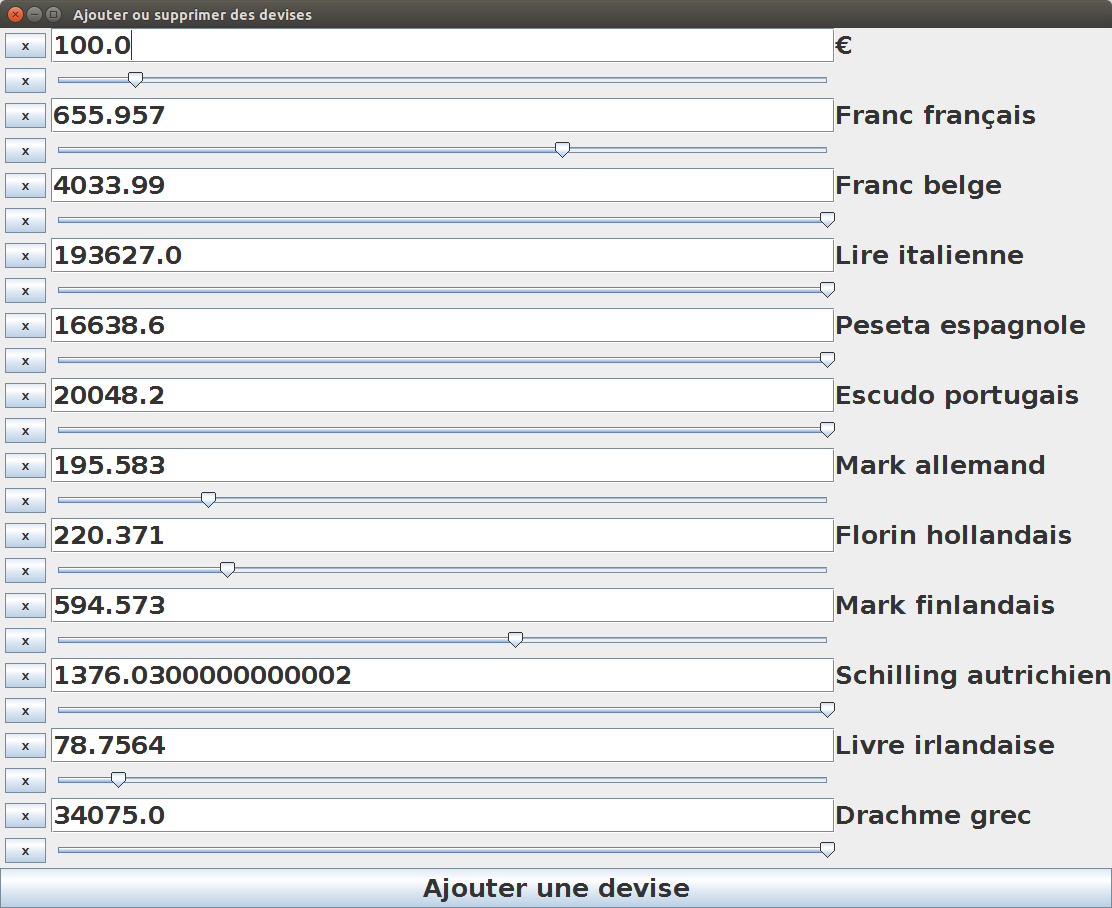
\includegraphics[width=\linewidth]{images/europe}

\vspace*{20mm}

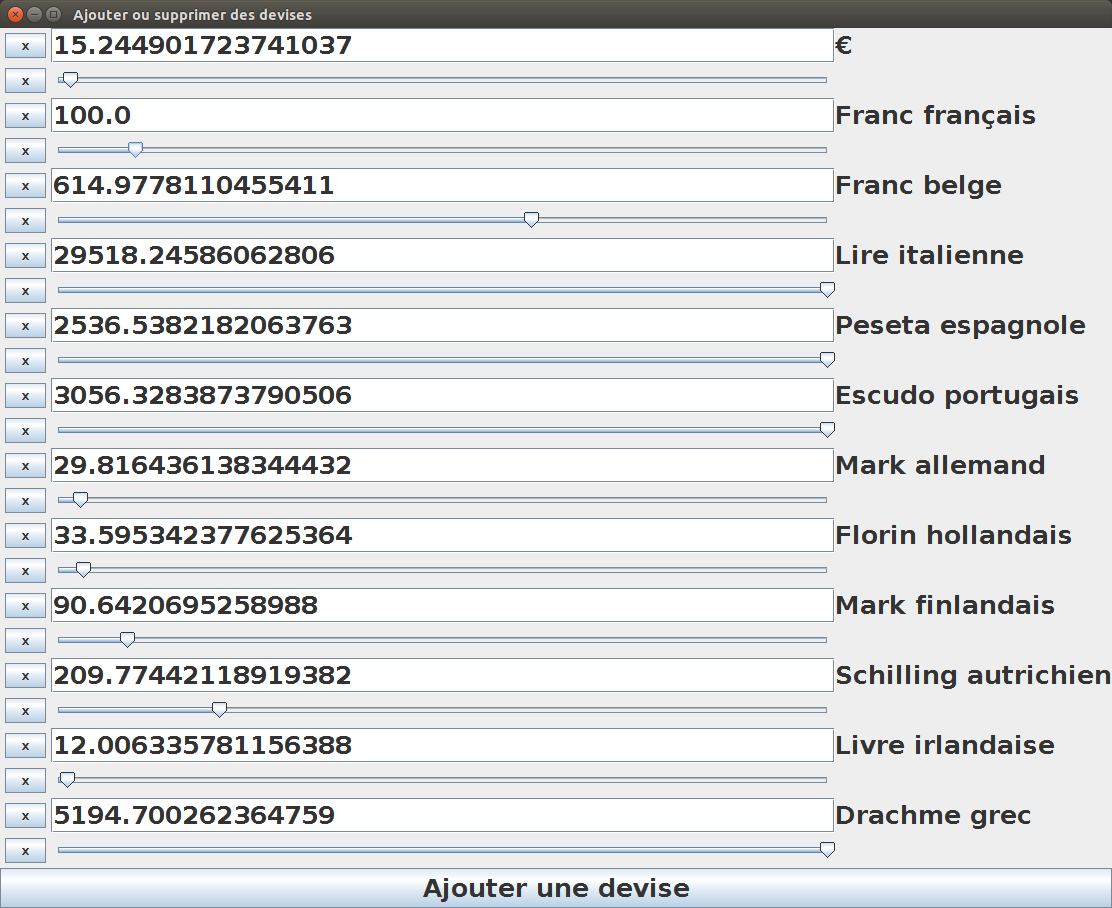
\includegraphics[width=\linewidth]{images/europe2}
\end{minipage}

\medskip

Pour r�aliser ce travail, il est pr�f�rable de mettre en \oe{}uvre le pattern Observer.

\medskip

Vous avez � votre disposition un projet Netbeans Java (\og PatronObservateurACompleter) qui fournit la trame. 









\end{document}


